% \documentclass[aspectratio=169]{beamer}
\documentclass[10pt]{beamer}
\usepackage[utf8]{inputenc}
\usepackage{beamerthemesplit}
\usepackage{url}
\usepackage{hyperref}
\usepackage{alltt}
\usepackage{lmodern}
\usepackage{wrapfig}

% \usetheme{Warsaw}
\usetheme{Frankfurt}
%\usecolortheme[RGB={132,186,75}]{structure}
\setbeamercolor{tableofcontents}{fg=red}
\setbeamerfont{structure}{series=\bfseries} 
\usecolortheme{seagull}
\useoutertheme[subsection=false]{smoothbars} % Beamer Outer Theme
\useinnertheme{rounded} % Beamer Inner Theme

\graphicspath{{images/}}

% \logo{\includegraphics[width=3cm]{cct_logo.png}}
\logo{
\includegraphics[width=2.0cm]{LA-SiGMA_Logo.jpg}}

\newcommand{\Hhybtwid}{\tilde{H}_\text{hyb}}
\newcommand{\Tr}{\text{Tr}}
% We want to use the infolines outer theme because it uses so less space, but
% it also tries to print an institution (which we do not have) and the slide
% numbers (which we might not want to show). Therefore, we here redefine the
% footline ourselfes - mostly a copy & paste from
% /usr/share/texmf/tex/latex/beamer/themes/outer/beamerouterthemeinfolines.sty
\defbeamertemplate*{footline}{infolines theme without institution and slide numbers}
{
  \leavevmode%
  \hbox{%
  \begin{beamercolorbox}[wd=.333333\paperwidth,ht=2.25ex,dp=1ex,center]{author in head/foot}%
    \usebeamerfont{author in head/foot}\insertshortauthor
  \end{beamercolorbox}%
  \begin{beamercolorbox}[wd=.333333\paperwidth,ht=2.25ex,dp=1ex,center]{title in head/foot}%
    \usebeamerfont{title in head/foot}\insertshorttitle
  \end{beamercolorbox}%
  \begin{beamercolorbox}[wd=.333333\paperwidth,ht=2.25ex,dp=1ex,center]{date in head/foot}%
    \usebeamerfont{date in head/foot}\insertshortdate{}
  \end{beamercolorbox}}%
  \vskip0pt%
}

% For some reason this is not displayed by default. This is just a copy & paste
% from the same file as the footline
\defbeamertemplate*{headline}{infolines theme with sections/subsections}
{
  \leavevmode%
  \hbox{%
  \begin{beamercolorbox}[wd=.5\paperwidth,ht=2.25ex,dp=1ex,right]{section in head/foot}%
    \usebeamerfont{section in head/foot}\insertsectionhead\hspace*{2ex}
  \end{beamercolorbox}%
  \begin{beamercolorbox}[wd=.5\paperwidth,ht=2.25ex,dp=1ex,left]{subsection in head/foot}%
    \usebeamerfont{subsection in head/foot}\hspace*{2ex}\insertsubsectionhead
  \end{beamercolorbox}}%
  \vskip0pt%
}

% some settings for captions
\setbeamertemplate{caption}{\raggedright\insertcaption\par}
\setbeamerfont{caption}{size=\scriptsize}
\title[TESC Seminar]{Continuous-time Quantum Monte Carlo - Hybridization-expansion Algorithm for Fermions (I)}
\author[Jian Tao]{Jian Tao}
\institute{Center for Computation \& Technology \\
Louisiana State University \\
\texttt{jtao@cct.lsu.edu}\\
\vspace{.25cm} Technologies for Extreme Scale Computing Seminar}
\date{April 9th, 2015 Baton Rouge, LA}
\begin{document}
\frame{\titlepage}

\section[Outline]{}
  \frame{\tableofcontents}
\section{Quantum Impurity Problems and Model}
  \frame { \frametitle{Quantum Impurity Problems}
\vspace{-20pt}  
  \begin{figure}
    \begin{center}
      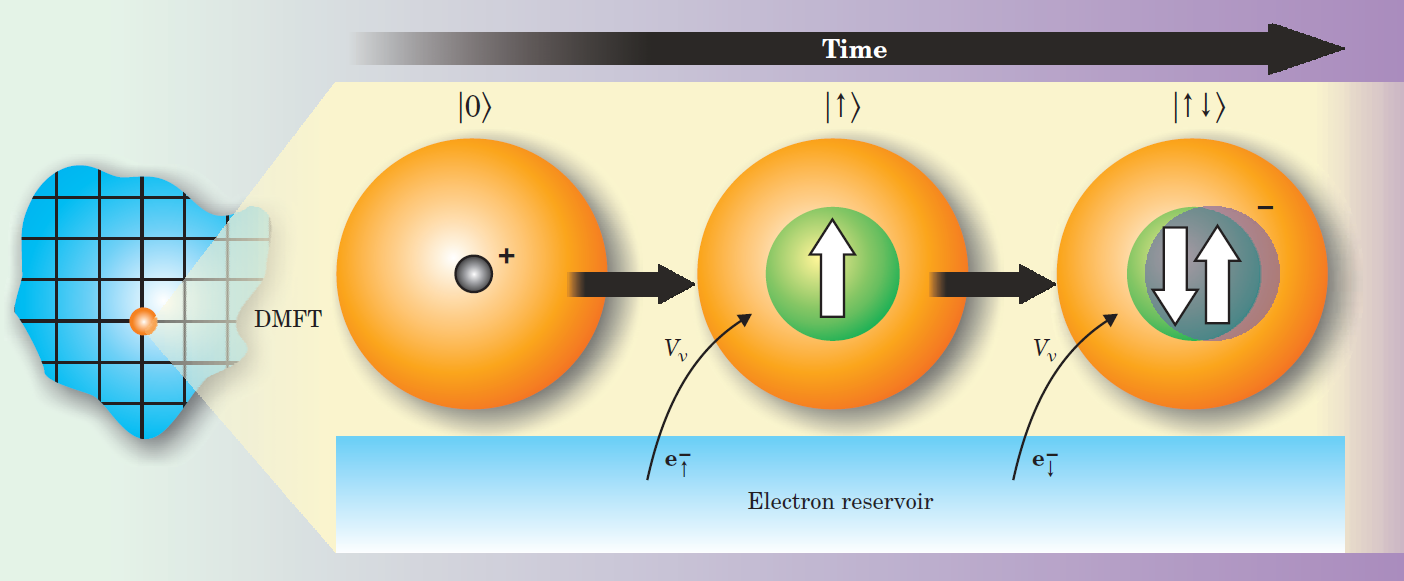
\includegraphics[width=0.8\textwidth]{qips.png}
      \vspace{-10pt}
        \caption{G. Kotliar and D. Vollhardt, Phys. Today March, 53 (2004)}
    \end{center}
  \end{figure}
\vspace{-20pt}
\begin{itemize}
 \item Quantum Impurity Problems(QIPs) were initially constructed to describe the quantum mechanical 
       properties of an impurity or imperfection such as 
       a magnetic atom, dislocation, or a substitutional ion in a lattice.
 \item Many-body lattice problems, such as heavy fermion systems, Mott metal-insulator transition, 
       nonconventional superconductivity could be mapped to QIPs with dynamical mean field theory (DMFT).
\end{itemize}
}

\frame { \frametitle{Quantum Impurity Model}
A quantum impurity model may be represented as a Hamiltonian $H_\text{QI}$

\begin{block}{$H_\text{QI}=H_\text{loc}+H_\text{bath}+H_\text{hyb}$}
\begin{eqnarray}
H_\text{loc}&=& H_\text{loc}^0+H_\text{loc}^I= \sum_{ab} E^{ab}d^\dagger_a d_b + \sum_{pqrs}I^{pqrs}d^\dagger_p d^\dagger_q d_r d_s \\
H_\text{bath}&=&\sum_{k\alpha} \varepsilon_{k\alpha}c^\dagger_{k\alpha}c_{k\alpha} \\
H_\text{hyb}&=&\sum_{k\alpha b} ({V}_k^{\alpha b}c^\dagger_{k\alpha}d_b +\text{h.c.})
\end{eqnarray}
\end{block}
$H_\text{loc}$ describes the ``impurity'' (a system
with a finite (typically small) number of degrees of freedom), 
$H_\text{bath}$ describes the noninteracting system, 
and $H_\text{hyb}$ gives the coupling between the impurity and bath.
}

\frame { \frametitle{Anderson Impurity Model}
The Anderson impurity model describes a localized electronic level, subject to a local Coulomb interaction, which
is coupled to a band of non-interacting conduction electrons.
In the  single-impurity single-orbital case, its Hamiltonian reads
\begin{block}{}

\begin{eqnarray}
H_\text{AIM}&=& \underbrace{\sum_{k\sigma}\varepsilon_k c^\dagger_{k\sigma}c_{k\sigma}}_{H_\text{bath}} 
             +  \underbrace{\sum_\sigma \varepsilon_0d^\dagger_\sigma d_\sigma +Un_\uparrow n_\downarrow}_{H_\text{loc}}\nonumber \\
            &+& \underbrace{\sum_{k\sigma}\Big(V_kc^\dagger_{k\sigma}d_\sigma+h.c.\Big)}_{H_\text{hyb}}
\end{eqnarray}

$\varepsilon_0$ is the level energy and $Un_\uparrow n_\downarrow$ is the interaction term.

\end{block}
}

\section{Overview of Continuous-time Quantum Monte Carlo Method}
  % \frame { \frametitle{Hirsch-Fye Quantum Monte Carlo Method}
% The Hirsch-Fye QMC (HF-QMC) was the  method of choice used to construct QIP 
% solvers before the Continuous-time QMC (CT-QMC).
% 
% HF-QMC writes the imaginary-time functional integral by discretizing
% the interval into $M$ equally spaced “time-slices” and then on each time-slice 
% applies a discrete Hubbard-Stratonovich transformation, as shown with the single 
% orbital Anderson impurity model,
% 
% \begin{align}
% e^{-\Delta \tau U\left(n_\uparrow 
% n_\downarrow-\frac{n_\uparrow+n_\downarrow}{2}\right)}&=\frac{1}{2}\sum_{
% s_i=\pm 
% 1}e^{\lambda s_i\left(n_\uparrow-n_\downarrow\right)},\\
% \lambda&=\text{arcosh}\left[\exp\left(\frac{1}{2}\Delta\tau U\right)\right].
% \end{align}
% }
% 
% \frame { \frametitle{CT-QMC vs HF-QMC}
% CT-QMC has several advantages over HF-QMC,
% 
% \begin{itemize}
% \item HF-QMC requires an equally spaced time discretization which may 
%       cause troubles in time step extrapolation while CT-QMC doesn't have such 
% issues by design.
% \item At large interactions and low temperatures, equilibration may become an 
% issue for HF-QMC while it could be handled in CT-QMC.
% \item For system beyong single orbital, it is prohibitively difficult to handle 
% with HF-QMC 
%       while CT-QMC could be generalized to handle multiple orbital cases.
% \end{itemize}
% }

\frame { \frametitle{Basic Idea of CT-QMC}
In CT-QMC, the Hamiltonian $H=H_a+H_b$ is split into two parts.
The partition function $Z=\Tr[e^{-\beta H}]$ is written in the interaction representation 
with respect to $H_a$ and expands in powers of $H_b$,
\begin{align}
Z=&\Tr\ {T_\tau} e^{-\beta H_a} \text{exp} \left[-\int_0^\beta d\tau H_b(\tau)\right] \nonumber \\
=&\sum_k (-1)^k\int_0^\beta d\tau_1\ldots\int_{\tau_{k-1}}^\beta d\tau_k \nonumber \\
&\times \text{Tr}\big[e^{-\beta H_a}H_b(\tau_k)H_b(\tau_{k-1})\ldots H_b(\tau_1)\big]
\end{align}
The impurity Green's function ($0 < \tau < \beta$) or the ``solution'' of the impurity model is then given by
\begin{equation}
 G(\tau) = \frac{1}{Z}\Tr[e^{-(\beta-\tau) H} d e^{-\tau H} d^\dagger]
\end{equation}
}

\frame { \frametitle{CT-QMC Expansion Algorithms}
There are several expansion algorithms with different choices of $H_b$. The most
widely used ones are:
\begin{itemize}
  \item CT-INT (Interaction expansion, $H_b=H^I_\text{loc}$): works well for clusters, single orbital models, 
  has sign problem with repulsive interactions, is not good for general electric structure Hamiltonians.
  \item CT-HYB (Hybridization expansion, $H_b=H_\text{hyb}$): works well for multi-orbital systems, 
  handles low temperature and strong interactions more efficiently, is not good for clusters.
\end{itemize}
Some other expansion algorithms that either consider an additional auxiliary field decomposition (for clusters) 
or exchange coupling (for Kondo problems) have been developed as well.
}  
\section{Hybridization-expansion Algorithm}
  \frame { \frametitle{Hybridization Expansion (I)}
In CT-HYB, we separate bath and impurity operators and obtain
\begin{align}
H_b&=H_\text{hyb} = \underbrace{\sum_{pj} (V_p^j c_{p}^\dagger d_j}_{\tilde{H}_\text{hyb}}  
+ \underbrace{\sum_{pj} V_p^{j*}d_j^\dagger c_{p})}_{\tilde{H}_\text{hyb}^\dagger} \\
Z &=\sum_{k=0}^\infty\int_0^\beta d\tau_1 \ldots \int_{\tau_{k-1}}^\beta d\tau_k \int_0^\beta d\tau_1' \ldots  \int_{\tau_{k-1}'}^\beta d\tau_k' \nonumber\\
&\sum_{\substack{j_1, \cdots j_k\\j_1', \cdots j_k'}}\sum_{\substack{p_1, \cdots p_k\\p_1',\cdots p_k'}} V^{j_1}_{p_1}V^{j_1'*}_{p_1'} \cdots V^{j_k}_{p_k}V^{j_k'*}_{p_k'}  \nonumber\\
&\times\Tr_d\left[T_\tau e^{-\beta H_\text{loc}} d_{j_k}(\tau_k) d_{j_k'}^\dagger(\tau_k')\cdots d_{j_1}(\tau_1)d_{j_1'}^\dagger(\tau_1')\right] \nonumber \\
&\times\Tr_c\left[T_\tau e^{-\beta H_\text{bath}} c^\dagger_{p_k}(\tau_k)c_{p_{k'}}(\tau_k')\cdots c_{p_1}^\dagger(\tau_1) c_{p_1'}(\tau_1')\right]
\end{align}
}

\frame { \frametitle{Hybridization Expansion (II)}
The bath partition function could be integrated out
\begin{align}
Z_\text{bath} = \Tr e^{-\beta H_\text{bath}} = \prod_\sigma \prod_{p} (1+e^{-\beta \varepsilon_{p}}),
\end{align}
With the anti-periodic hybridization function $\mathbf{\Delta}$,
\begin{align}
\Delta_{lm}(\tau) = \sum_p \frac{V^{l*}_p V^m_p}{e^{\varepsilon_p\beta}+1} \times \left\{ \begin{array}{ll}-e^{-\varepsilon_p(\tau-\beta)},& 0<\tau<\beta \\ e^{-\varepsilon_p\tau},&  -\beta<\tau<0\end{array}\right.,
\end{align}
and by separating the contributions from each spin, we obtain
\begin{eqnarray}
\label{partition_function}
Z &=&  Z_\text{bath}\prod_j \sum_{k_j=0}^\infty \int_0^\beta d\tau^j_1 \ldots \int_{{\tau'}^j_{k_j-1}}^\beta d{\tau'}^j_{k_j} \\
&\times& \Tr_d\Big[T_\tau e^{-\beta H_\text{loc}} d_j(\tau^j_{k_j}) d_j^\dagger(\tau'^j_{k_j})\ldots d_j(\tau^j_{1})d_j^\dagger(\tau'^j_1)\Big] \det \mathbf{\Delta}_j.\nonumber
\end{eqnarray}
}
\section{Diagrammatic Monte Carlo}
  \frame { \frametitle{Monte Carlo Method}
Monte Carlo methods are the only practical choices to do very high dimension integrations such as 
equation~\ref{partition_function}.

For $x \in\mathcal{C}$ with weight $p(x)$, we have the partition function
\begin{equation}
Z=\int_{C} dx~p(x)
\end{equation}

The expectation value of a quantity A is given by
\begin{equation}
 \langle A \rangle_{p} = \frac{1}{Z}\int_{C} dx~A(x)p(x)
\end{equation}

With $M$ configurations $x_i$ in a Monte Carlo procedure,

\begin{equation}
\langle A \rangle_p \approx \langle A \rangle_{MC} \equiv \frac{1}{M}\sum_{i=1}^M {A}(x_i).
\end{equation}

}

\frame { \frametitle{Markov Process}

A Markov process defines a transition matrix $W_{xy}$ which specifies 
the probability to go from state $x$ to state $y$ in one step of 
the Markov process.

The Markov process will converge exponentially from any initial state to a stationary distribution $p(x)$ 
if two conditions are satisfied.
\begin{block}{}
\begin{itemize}
\item Ergodicity: for all $x$ and $y$ there exists an integer $N<\infty$ such that for all $n\ge N$ the probability  $(W^n)_{xy}\ne 0$.
\item Balance: the distribution $p(x)$ satisfies the detailed balance condition
\begin{align}
\frac{W_{xy}}{W_{yx}} = \frac{p(y)}{p(x)} \nonumber
\end{align}
\end{itemize}
\end{block}
}

\frame { \frametitle{Metropolis-Hastings Algorithm}
An update from a configuration $x$ to a new configuration $y$ is proposed with a probability 
$W_{xy}^{\text{prop}}$ but accepted only with probability $W_{xy}^{\text{acc}}$.  
If the proposal is rejected  the old configuration $x$ is used again.

\begin{equation}
 W_{xy}^{\text{acc}}= \min\left[ 1,  \frac{p(y) W_{yx}^{\text{prop}}}{p(x) W_{xy}^{\text{prop}}} \right].
\end{equation}
\begin{align}
W_{xy} &= W_{xy}^{\text{prop}}W_{xy}^{\text{acc}}
\end{align}
}

\frame { \frametitle{Hybridization Update Diagrams}
(a) original configuration; (b) removal of a segment; (c) shift of an end point of a segment; (d) insertion of an antisegment; (e) removal of an antisegment; (f) removal of another antisegment such that the remaining segment "wraps" around $\beta$.
\begin{figure}
    \begin{center}
      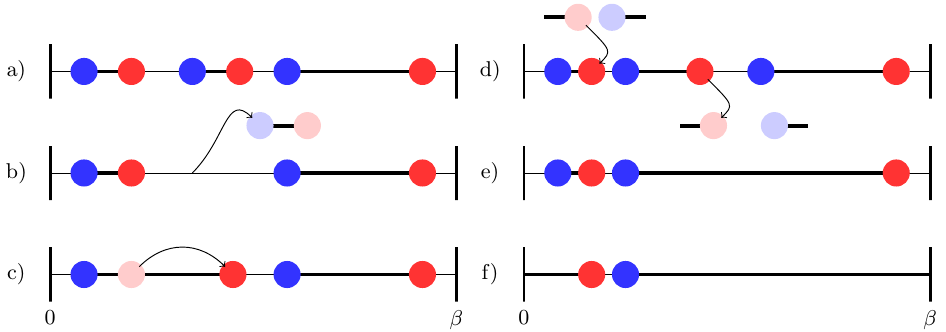
\includegraphics[width=0.95\textwidth]{hyb_diagrams.png}
    \end{center}
  \end{figure}
}

\frame { \frametitle{Segment Representation}
Segment representation make it possible to treat interaction by looking at overlap of lines.
Extension to density - density interactions for multiple orbitals
is made straightforward as well.
\\
\begin{figure}
    \vspace{20pt}
    \begin{center}
      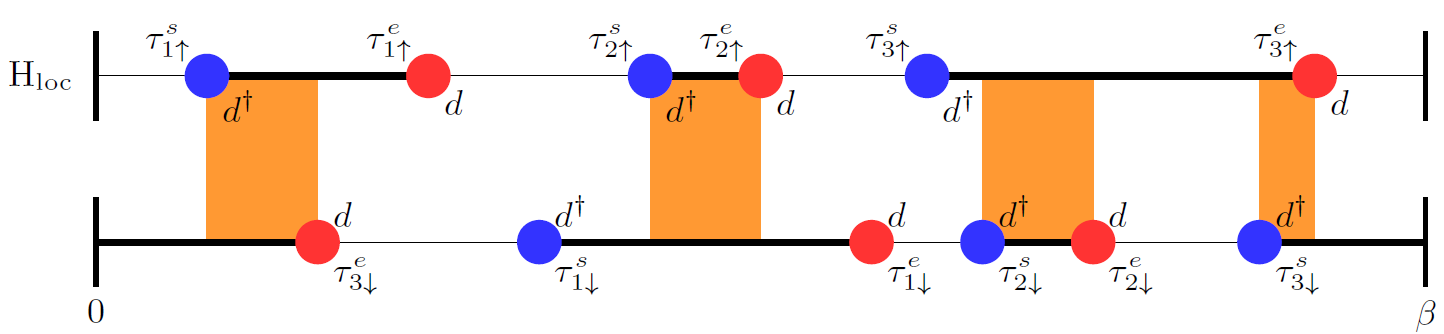
\includegraphics[width=0.95\textwidth]{segment}
    \end{center}
  \end{figure}
}

\frame { \frametitle{Segment Representation}
Possible hybridization lines of a particular segment configuration.
\\
\begin{figure}
    \begin{center}
      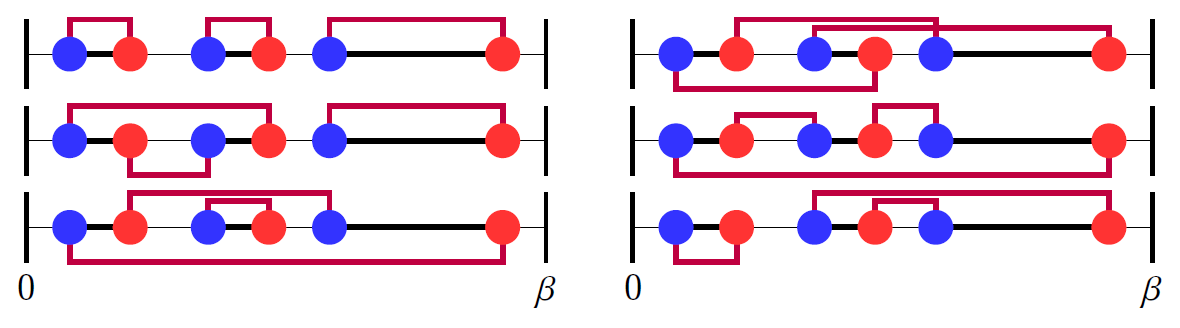
\includegraphics[width=0.9\textwidth]{hybridization_lines}
    \end{center}
    \vspace{-20pt}
  \end{figure}
}


\frame { \frametitle{CTQMC Workflow}
  \begin{figure}
    \begin{center}
      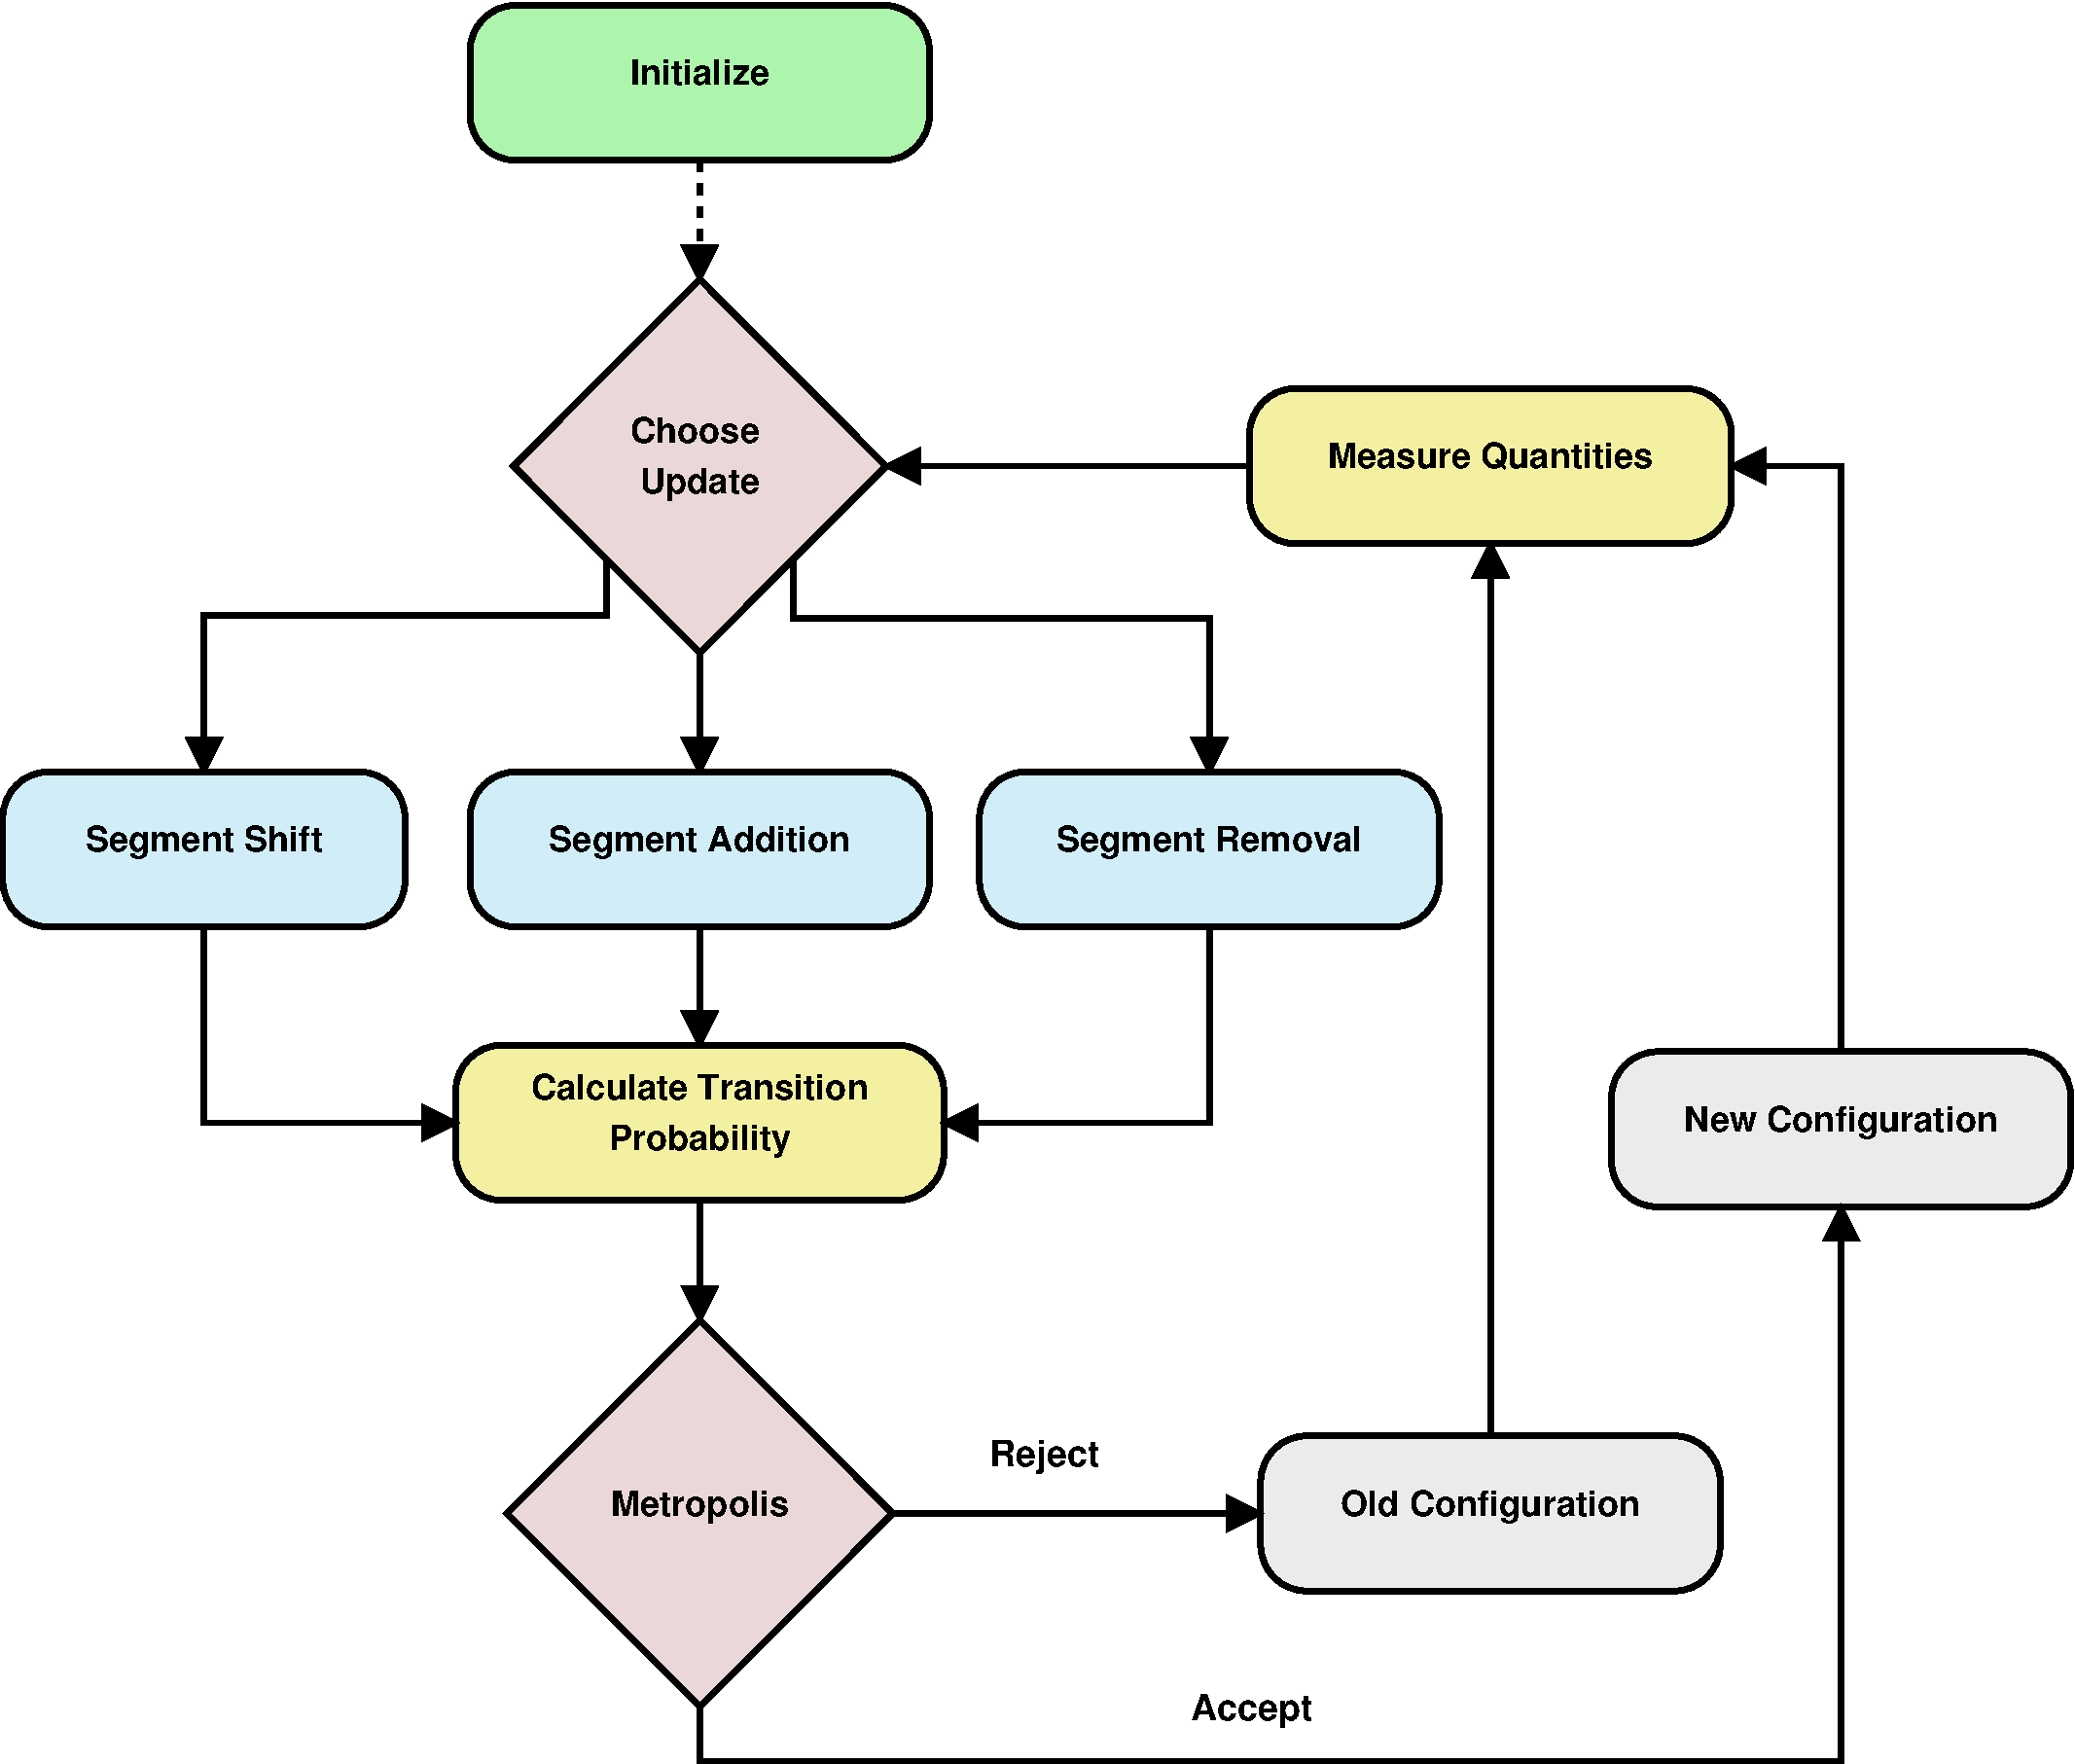
\includegraphics[height=0.7\textwidth]{CTQMC}
    \end{center}
  \end{figure}
}  
\section{Acknowledgments}
  \frame { \frametitle{Acknowledgment}
\begin{block}{My thanks go to}
\begin{itemize}
  \item Sheng Feng, Ka-Ming Tam, and Shuxiang Yang for discussions and help.
  \item Mark Jarell and Juana Moreno for support and encouragement.
\end{itemize}
\end{block}
\begin{block}{}
This material is based upon work supported by the National Science Foundation 
under the NSF EPSCoR Cooperative Agreement No. EPS-1003897 with additional 
support from the Louisiana Board of Regents.
\end{block}
}
\section{References}
  \frame { \frametitle{References}
\begin{itemize}
  \item Werner, P., Comanac, A., De’Medici, L., Troyer, M., \& Millis, A. J. 
(2006). Continuous-time solver for quantum impurity models. Physical review 
letters, 97(7), 076405.
  \item Werner, P., \& Millis, A. J. (2006). Hybridization expansion impurity 
solver: General formulation and application to Kondo lattice and two-orbital 
models. Physical Review B, 74(15), 155107.
  \item Gull, E., Millis, A. J., Lichtenstein, A. I., Rubtsov, A. N., Troyer, 
M., \& Werner, P. (2011). Continuous-time Monte Carlo methods for quantum 
impurity models. Reviews of Modern Physics, 83(2), 349.
  \item Annam\'{a}ria Kiss, Note on the continuous-time quantum Monte Carlo (CT-QMC)
simulation method, December 23, 2009.
  \item iQIST: An open source continuous-time quantum Monte
Carlo impurity solver toolkit (\url{http://arxiv.org/pdf/1409.7573.pdf}).
\end{itemize}
}
\end{document}
